\documentclass[logo,reportComp]{thesis}
\usepackage[cpp,pseudo]{mypackage}

\title{操作系统原理实验报告}
\subtitle{实验十:文件系统}
\school{数据科学与计算机学院}
\author{陈鸿峥}
\classname{17大数据与人工智能}
\stunum{17341015}
\headercontext{操作系统原理实验报告}
% \authorremark{本实验报告用\LaTeX撰写,创建时间:\builddate\today}

\begin{document}

\maketitle

\section{实验目的}
\begin{itemize}
	\item 学习文件操作的方法,掌握其实现方法。
	\item 利用FAT12文件系统实现原型操作系统的文件管理控制命令。
	\item 扩展MyOS的系统调用,实现进程中文件创建、文件打开、文件读、文件写和文件关闭等。
\end{itemize}

\section{实验要求}
% 实验目的和实验要求由老师提供实验项目文档中获取
原型保留原有特征的基础上,设计满足下列要求的新原型操作系统:
\begin{enumerate}
\item 参考DOS的命令功能,实现文件管理控制命令\verb'cd'、\verb'dir'、\verb'del'、\verb'copy'等。
\item 扩展MyOS的系统调用,在C语言中,程序可以调用文件创建、文件打开、文件读、文件写和文件关闭等系统调用。
\item 编写一个测试的这些系统调用的C语言用户程序,编译产生可执行程序进行测试。
\end{enumerate}

\section{实验环境}
% 包括:硬件或虚拟机配置方法、软件工具与作用、方案的思想、相关原理、程序流程、算法和数据结构、程序关键模块,结合代码与程序中的位置进行解释。不得抄袭,否则按作弊处理。
% 实验方案包括相关基础原理、实验工具和环境、程序流程和算法思想、数据结构与程序模块功能说明,代码文档组成说明等
具体环境选择原因已在实验一报告中说明。
\begin{itemize}
	\item Windows 10系统 + Ubuntu 18.04(LTS)子系统
	\item gcc 7.3.0 + nasm 2.13.02 + GNU ld (Binutils) 2.3.0
	\item GNU Make 4.1
	\item Oracle VM VirtualBox 6.0.6
	\item Bochs 2.6.9
	\item Sublime Text 3 + Visual Studio Code 1.33.1
\end{itemize}

虚拟机配置:内存4M,1.44M虚拟软盘引导,1.44M虚拟硬盘。

\section{实验方案}
% 包括:主要工具安装使用过程及截图结果、程序过程中的操作步骤、测试数据、输入及输出说明、遇到的问题及解决情况、关键功能或操作的截图结果。不得抄袭,否则按作弊处理。
{\textbf{\textcolor{red}{本次实验继续沿用实验六保护模式的操作系统。用户程序都以ELF文件格式读入,并且在用户态(ring 3)下执行。}}}

\subsection{FAT12文件系统}
由于虚拟出来的硬盘容量较小,且没有那么多数据需要管理,故本实验采用FAT12文件系统。

\subsubsection{基本理论}
针对1.44M的虚拟软盘/硬盘,FAT12将其划分为如图\ref{fig:disk}所示的几个部分。
\begin{figure}[H]
\centering
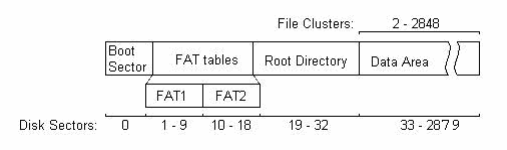
\includegraphics[width=0.6\linewidth]{fig/disk_organization.png}
\caption{FAT12磁盘划分\protect\footnote{图源自\url{http://www.disc.ua.es/~gil/FAT12Description.pdf}}}
\label{fig:disk}
\end{figure}
\begin{itemize}
	\item 引导程序区:0-1扇区
	\item 文件分配表(File Allocation Table)1:1-9扇区
	\item 文件分配表2:10-18扇区
	\item 根目录:19-32扇区
	\item 文件数据区:33扇区以后
\end{itemize}

注意上述所指的都是逻辑扇区。

对于\textbf{引导程序区},我用C的结构体封装了其各个字节的语义,如下。
\begin{lstlisting}
// Boot Sector (BS) & BPB (BIOS Parameter Block)
typedef struct bootsect
{
	uint8_t	      Jump[3]; // 3
	char          BS_OEMName[8]; // 11
	uint16_t      BPB_BytesPerSector; // 13
	uint8_t       BPB_SectorsPerCluster; // 14
	uint16_t      BPB_ReservedSectors; // 16
	uint8_t       BPB_NumFATs; // 17
	uint16_t      BPB_RootDirectoryEntries; // 19
	uint16_t      BPB_LogicalSectors; // 21
	uint8_t       BPB_MediumDescriptorByte; // 22
	uint16_t      BPB_SectorsPerFat; // 24
	uint16_t      BPB_SectorsPerTrack; // 26
	uint16_t      BPB_NumHeads; // 28
	uint32_t      BPB_HiddenSectors; // 32
	uint8_t       code[480]; // the last 2B is signature "AA55h"

} __attribute__ ((packed)) bootsect_t;
\end{lstlisting}

\textbf{文件分配表}即所谓的FAT,是一个数组模拟的链表,存放文件的组织方式。
由于用12位二进制位表示一个簇(cluster)的下标\footnote{FAT12中一个簇与一个扇区大小相同},故称为FAT12文件系统。
如图\ref{fig:fat}所示,由于FAT12涉及到半字节的处理,故会比较麻烦。
通常是3字节3字节进行处理,图\ref{fig:fat}的上图是物理FAT结构,下图是逻辑FAT结构,需要经过映射才得到真正的FAT。
\begin{figure}[H]
\centering
\begin{tabular}{c}

\includegraphics[width=0.6\linewidth]{fig/fat_1.jpg}\\
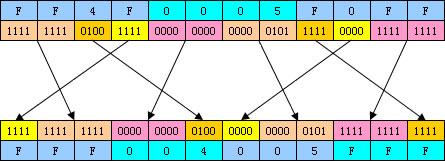
\includegraphics[width=0.6\linewidth]{fig/fat_2.jpg}
\end{tabular}
\caption{文件分配表\protect\footnote{图源自\url{http://blog.sina.com.cn/s/blog_3edcf6b80100crz1.html}}}
\label{fig:fat}
\end{figure}

前面三个字节\verb'F0 FF FF'是存储介质和标识符,故实际的文件存储从2号簇开始。
FAT数组内存放的内容指向下一个簇的下标,如果是\verb'0F00'-\verb'0FF7'则代表坏簇(文件结尾)。

如一个文件1000B,需要占用2个簇/扇区,则一种可能的方式是
\begin{lstlisting}
Index | 0   | 1   | 2   | 3   |
FAT   | FF0 | FFF | 003 | FF7 |
\end{lstlisting}

在C头文件中我分别创建了物理和逻辑两个不同的结构体
\begin{lstlisting}
typedef struct phys_fat
{
	uint8_t entry [FAT_PHYS_SIZE * FAT_SECTOR_SIZE]; // 4608

} __attribute__ ((packed)) phys_fat12_t;
static phys_fat12_t phys_fat;

typedef struct logic_fat
{
	// only the first 3B are used (24bits)
	// the first two clusters (0,1) are useless
	uint32_t entry [FAT_NUM_ENTRY]; // 3072

} __attribute__ ((packed)) fat12_t;
static fat12_t fat;
\end{lstlisting}

接着是\textbf{文件目录项},如图\ref{fig:directory}所示。
\begin{figure}[H]
\centering
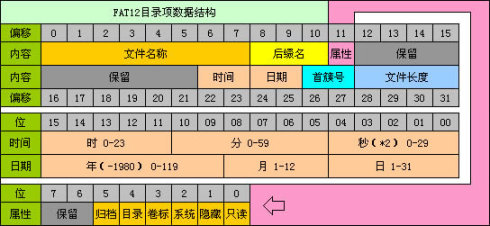
\includegraphics[width=0.6\linewidth]{fig/fat12_directory_entry.jpg}
\caption{FAT12文件目录项\protect\footnote{图源自\url{http://blog.sina.com.cn/s/blog_3edcf6b80100crz1.html}}}
\label{fig:directory}
\end{figure}

同样可以创建对应的结构体\verb'FileEntry',由于图\ref{fig:directory}已经十分清晰,这里不再赘述。
但注意日期、时间与整型的转换,我在\verb'fat12.h'头文件中创建了四个辅助函数来帮助转换。

最后是\textbf{根目录},一共有224项。
\begin{lstlisting}
typedef struct root_directory
{
	FileEntry_t entry[FAT_SECTOR_SIZE / sizeof(FileEntry_t) * FAT_ROOT_SIZE]; // 224

} __attribute__ ((packed)) fat_root_t;
static fat_root_t root_dir;
\end{lstlisting}

在FAT12文件系统中,目录与文件都是一个\verb'entry',只是属性不同,都至少占用一个簇。
而子目录将存储在数据区中,一个簇最多存储16项(因每个项占32B)。

下面将详细叙述具体的文件操作指令实施,由于是Linux环境,故对应的都是Linux的命令行语句的实施。
\subsubsection{文件系统初始化}
按照上述四个部分次序依次将FAT12的头部读入内存,同时设置了当前目录/簇\verb'curr_dir'和当前路径\verb'curr_path',方便索引。
由于一开始在根目录,故初始化\verb'curr_path'为\verb'"/"'。
\begin{lstlisting}
bool fat12_init()
{
	// Boot sector
	read_sectors((uintptr_t)&bootsector,FAT_BOOTSECTOR_START,FAT_BOOTSECTOR_SIZE);

	// FAT sectors
	read_sectors((uintptr_t)&phys_fat,FAT_ENTRY_START,FAT_PHYS_SIZE);

	// Converts the FAT into the logical structures (array of word).
	for (int i = 0, j = 0; i < 4608; i += 3)
	{
		fat.entry[ j++ ] = (phys_fat.entry[i] + (phys_fat.entry[i+1] << 8)) & 0x0FFF;
		fat.entry[ j++ ] = (phys_fat.entry[i+1] + (phys_fat.entry[i+2] << 8)) >> 4;
	}

	// root directory
	read_sectors((uintptr_t)&root_dir,FAT_ROOT_REGION_START,FAT_ROOT_SIZE);

	// set current path
	curr_dir = FAT_ROOT_REGION_START;
	strcpy(curr_path,"/");

	return true;
}
\end{lstlisting}

\subsubsection{目录查看}
目录查看对应的是Linux中的\verb'ls'指令。

首先实施\verb'fat12_show_file_entry',将对应的\verb'FileEntry_t* f'输出。
由于主要是字符串输出操作,故这里不再展示,但注意只有文件和目录需要输出,对于删除的文件\verb'name'首字节为\verb'0xE5'的也不需要展示。

由于根目录与其他子目录大小不同,故需要分别处理,下面的操作也是类似,需要注意。
\begin{lstlisting}
void fat12_ls()
{
	if (curr_dir == FAT_ROOT_REGION_START)
		for (int i = 0; i < FAT_NUM_ROOT_ENTRY; ++i)
			fat12_show_file_entry(&root_dir.entry[i]);
	else
		for (int i = 0; i < FAT_NUM_DIR_ENTRY; ++i)
			fat12_show_file_entry(&subdir.entry[i]);
}
\end{lstlisting}

\subsubsection{目录切换}
目录切换对应的是Linux中的\verb'cd'指令。

首先需要实施\verb'curr_dir'和\verb'curr_dir'的重赋值。
\begin{lstlisting}
void fat12_set_dir(int new_dir, char* action)
{
	if (curr_dir == FAT_ROOT_REGION_START){
		curr_dir = new_dir;
		strcpy(curr_path,"/");
		strcat(curr_path,action);
	} else {

		if (new_dir == 0)
			new_dir = FAT_ROOT_REGION_START;
		curr_dir = new_dir;

		if (strcmp(action,".") == 0)
			; // do nothing
		else if (strcmp(action,"..") == 0) {
			reverse(curr_path);
			char* tmp_path = curr_path;
			strsep(&tmp_path,"/");
			reverse(tmp_path);
			strcpy(curr_path,tmp_path);
			if (curr_dir == FAT_ROOT_REGION_START)
				strcpy(curr_path,"/");
		} else {
			strcat(curr_path,"/");
			strcat(curr_path,action);
		}
	}
}
\end{lstlisting}

然后找到对应的目录项,并将该目录项对应的簇读入内存。
注意\verb'.'和\verb'..'在FAT文件系统中也对应着一个项,即与其他文件/文件夹没有区别。
\begin{lstlisting}
bool fat12_cd(char* folder)
{
	FileEntry_t* fe = fat12_find_entry(folder);
	if (fe == NULL){
		put_error("No such file or directory!");
		return false;
	}
	fat12_set_dir(fe->startCluster,folder);
	fat12_read_clusters((char*)&subdir,fe->startCluster);
	return true;
}
\end{lstlisting}

\subsubsection{文件读入}
这是执行用户程序的关键,对每一个目录项的名字都进行匹配,如果匹配上则读取文件内容。
由于前两个簇不适用,故簇号到实际的硬盘逻辑扇区号需要经过\verb'clust+FAT_DATA_REGION_START-2'进行转换。
\begin{lstlisting}
// start from the @cstart-th cluster, read the whole file to @buf
// return the number of bytes read
int fat12_read_clusters(char* buf, uint32_t cstart)
{

	int i;
	uint32_t clust = cstart;
	for (i = 0; true; ++i)
	{
		uintptr_t addr = (uintptr_t) buf + i * FAT_SECTOR_SIZE;
		// remember to recalculate cstart
		read_sectors(addr, clust + FAT_DATA_REGION_START - 2, 1);
		enable();
		if (fat12_next_sector(&clust, clust) == false)
			break;
	}
	return i;
}

bool fat12_read_file(char* filename, char* addr, int* size)
{
	for (int i = 0; i < FAT_NUM_ROOT_ENTRY; ++i){
		char entry_name[13]; // with dot(.)!
		fat12_construct_file_name(entry_name,&root_dir.entry[i]);
		if (strcmp(filename,entry_name) != 0)
			continue;
		fat12_read_clusters(addr,root_dir.entry[i].startCluster);
		if (size != NULL)
			*size = root_dir.entry[i].fileLength;
		return true;
	}

	put_error("FAT No this file!");

	return false;
}
\end{lstlisting}

\subsubsection{文件删除}
删除操作对应Linux中的\verb'rm'指令。

删除的操作较为麻烦,虽然只需将目录项的\verb'name'第0个字节设为\verb'0xE5'即可,但需要重新写回磁盘。
同时,FAT对应的簇也应改为坏簇,也要写回磁盘
\begin{lstlisting}
bool fat12_rm(char* filename)
{
	FileEntry_t* fe = fat12_find_entry(filename);
	if (fe == NULL){
		put_error("No such file or directory!");
		return false;
	}
	fe->name[0] = 0x000000E5;
	if (curr_dir == FAT_ROOT_REGION_START)
		write_sectors((uintptr_t)&root_dir,FAT_ROOT_REGION_START,FAT_ROOT_SIZE);
	else
		fat12_write_clusters((char*)&subdir,curr_dir);
	fat12_del_fat_entry(fe->startCluster);
	return true;
}
\end{lstlisting}

\subsubsection{文件创建}
文件的创建则较为繁琐,按照如下流程:
\begin{enumerate}
	\item 计算需要多少个簇,记为\verb'numCluster'
	\item 从FAT中寻找\verb'numCluster'个未用的簇,同时记录下头地址,并创建起整个链表串
	\item 边创建FAT也要边将文件对应的内容写入对应的簇/扇区中
	\item 最后修改目录项,将文件信息填入
\end{enumerate}
碍于时间关系,这里修改过的内容都会被直接写入硬盘,尽管效率不是很高。
\begin{lstlisting}
void fat12_create_file(uintptr_t addr, int size, char* name)
{
	int numCluster = (size % FAT_SECTOR_SIZE == 0 ?
		size / FAT_SECTOR_SIZE :
		size / FAT_SECTOR_SIZE + 1);

	int cnt = 0, prevIndex = -1, cstart = 0;
	for (int i = 2; i < FAT_NUM_ENTRY; ++i) // do NOT start from 0!
		if (fat.entry[i] == 0){
			if (cnt == 0)
				cstart = i;
			if (prevIndex != -1)
				fat.entry[prevIndex] = i;
			prevIndex = i;
			write_sectors(addr+i*FAT_SECTOR_SIZE,i+FAT_DATA_REGION_START-2,1);
			cnt++;
			if (cnt == numCluster){
				fat.entry[i] = 0x0FFF;
				break;
			}
		}
	fat12_write_back_fat();

	for (int i = 0; i < FAT_NUM_ROOT_ENTRY; ++i)
		if (root_dir.entry[i].name[0] == 0x00000000){
			char tmp_name[20];
			strcpy(tmp_name,name);
			char* ext = tmp_name;
			strsep(&ext,".");
			strcpy(root_dir.entry[i].name,tmp_name);
			for (int j = strlen(root_dir.entry[i].name); j < 8; ++j)
				root_dir.entry[i].name[j] = ' ';
			strcpy(root_dir.entry[i].extension,ext);
			for (int j = strlen(root_dir.entry[i].extension); j < 3; ++j)
				root_dir.entry[i].extension[j] = ' ';
			root_dir.entry[i].attribute.archive = true;
			root_dir.entry[i].startCluster = cstart;
			root_dir.entry[i].fileLength = size;
			root_dir.entry[i].date = date_to_int(2019,6,23);
			root_dir.entry[i].time = time_to_int(0,0,0);
			break;
		}
	write_sectors((uintptr_t)&root_dir,FAT_ROOT_REGION_START,FAT_ROOT_SIZE);
}
\end{lstlisting}
% 只实现在根目录下的创建

\subsubsection{文件复制}
复制对应着Linux的\verb'cp'指令。

有了前面文件创建的基础,文件复制实施起来就很简单了。
只需读取文件,然后拷贝一份写入即可。
\begin{lstlisting}
bool fat12_cp(char* src, char* dst)
{
	char buf[512 * 30];
	int size = 0;
	if (fat12_read_file(src,buf,&size)){
		fat12_create_file((uintptr_t)buf,size,dst);
		return true;
	}
	return false;
}
\end{lstlisting}

\subsection{虚拟文件系统}
这一部分是文件系统更高层的抽象管理,更加方便C用户程序的调用。
这里文件系统采用\verb'int 0x82'号中断,已经做了API的封装。

对于文件管理,我创建了如下的结构体,同时创建了一个维护文件的全局数组\verb'file_list'。
\begin{lstlisting}
typedef struct _FILE {

	char        name[32];
	char        mode[4];
	char        buffer[1024];
	char*       pos;
	uint32_t    fileLength;
	uint32_t    startCluster;
	uint32_t    currentCluster;

}FILE, *PFILE;

static FILE file_list[MAX_FILE_NUM];
\end{lstlisting}

\subsubsection{文件打开与关闭}
文件打开首先要判断文件是否存在,如果文件不存在,且为写模式,则创建新文件。
然后将文件对应的簇读入到文件结构体的缓冲数组中。

为避免频繁的硬盘读写,故文件内容都是统一读入\verb'buffer'进行处理,然后在文件关闭时再将\verb'buffer'内容写回硬盘。
\begin{lstlisting}
FILE* do_fopen(const char *pname, const char *mode)
{
	FILE* file = NULL;
	for (int i = 0; i < MAX_FILE_NUM; ++i)
		if (strcmp(file_list[i].mode,"u") == 0){
			file = &file_list[i];
			break;
		}
	if (file == NULL)
		return NULL;
	strcpy(file->name,pname);
	FileEntry_t* fe = fat12_find_entry((char*)pname);
	if (fe == NULL && strcmp(mode,"w") == 0){
		strcpy(file->mode,mode);
		return file;
	} else if (fe == NULL && strcmp(mode,"r") == 0)
		return NULL;
	file->fileLength = fe->fileLength;
	file->currentCluster = file->startCluster = fe->startCluster;
	strcpy(file->mode,mode);
	fat12_read_clusters(file->buffer,file->startCluster);
	return file;
}

int do_fclose(FILE* fp)
{
	if (strcmp(fp->mode,"w") == 0)
		fat12_create_file((uintptr_t)fp->buffer,fp->pos-fp->buffer,fp->name);
	strcpy(fp->mode,"u");
	enable();
	return 0;
}
\end{lstlisting}

\subsubsection{文件读写}
我实现了以下几个函数,都比较简单,主要是内存的操作。
\begin{lstlisting}
int do_fread(void *buf, int size, int count, FILE *fp)
{
	int numBytes = size * count;
	memcpy((char*)buf,fp->buffer,numBytes);
	return count;
}

int do_fwrite(void *buf, int size, int count, FILE *fp)
{
	if (strcmp(fp->mode,"w") != 0)
		return 0;
	int numBytes = size * count;
	memcpy(fp->pos,(const char*)buf,numBytes);
	fp->pos = fp->pos + numBytes;
	return count;
}

char *do_fgets(char *str, int count, FILE *fp)
{
	memcpy((char*)str,fp->buffer,count);
	return str;
}

int do_fputs(const char *str, FILE *fp)
{
	if (strcmp(fp->mode,"w") != 0)
		return 0;
	memcpy(fp->pos,str,strlen(str));
	fp->pos = fp->pos + strlen(str);
	return 1;
}
\end{lstlisting}

% 打开文件表
% 每个进程一份
% 每个打开的文件一行
% 记录本文件的打开方式、读写位置和指向活动文件记录

% 活动文件表
% 管理系统中所有打开的文件(一份)
% 每个打开的文件一个记录
% 记录本文件的目录项中的信息、缓冲块队列和共享控制位和共享计数等等

% 缓冲池
% 系统内核中利用一组内存块存放从文件中读取或准备写入的扇区
% 文件读操作会先在缓冲队列中找,命中则省了读磁盘,加快响应
% 文件写操作会先在缓冲队列中进行,关闭文件或系统内核定时写回磁盘,减少I/O次数,加快响应。

\section{实验结果}
我将所有的用户程序都放入创建的虚拟硬盘中\footnote{利用Linux的mount语句可以把虚拟硬盘挂载后,然后很方便地执行文件操作。},并创建了两个测试目录,如图\ref{fig:zip}所示。
\begin{figure}[H]
\centering
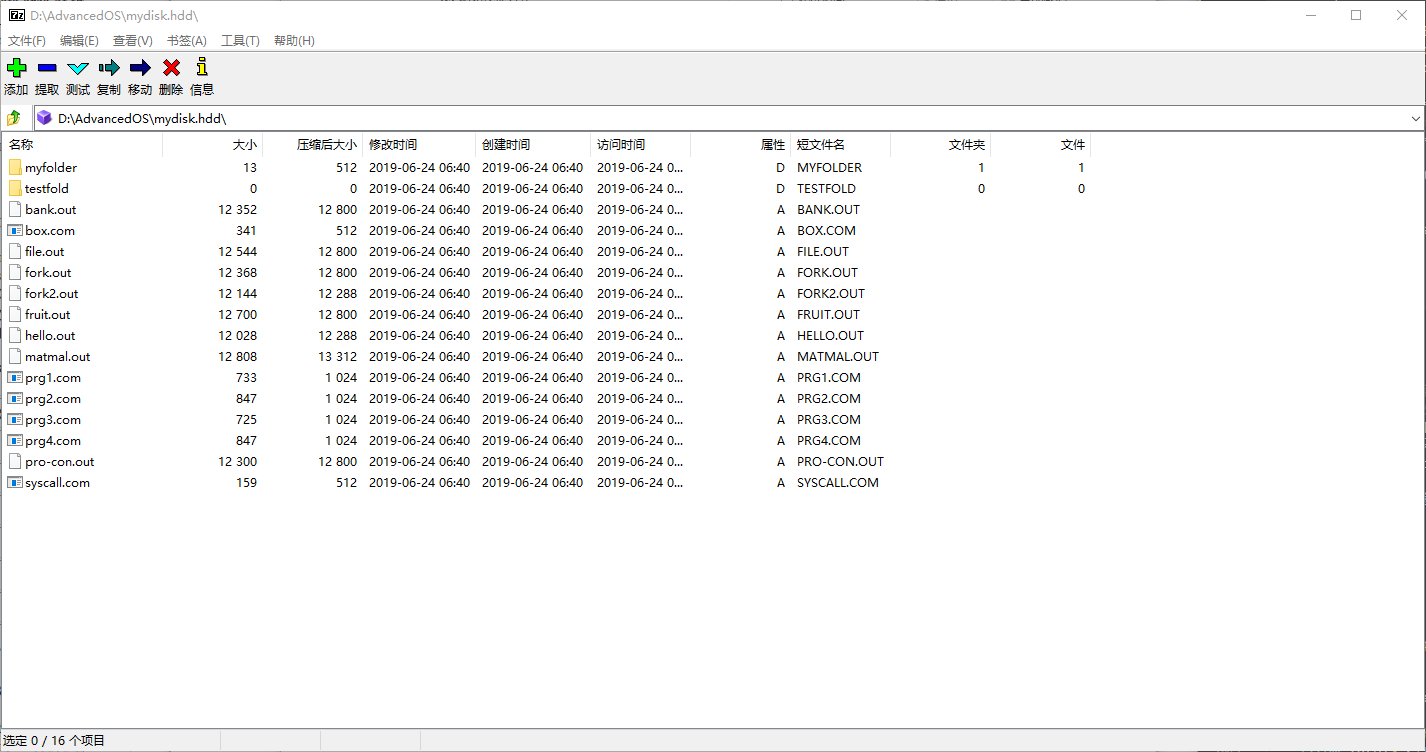
\includegraphics[width=0.8\linewidth]{fig/zip.png}
\caption{用7ZIP查看虚拟硬盘内容}
\label{fig:zip}
\end{figure}

从图\ref{fig:dir}中可以看到,随着目录的切换,前面的文件夹显示也会跟着改变。
向下的文件夹索引及向上的\verb'..'文件夹索引也都没有问题。
同时,想要访问不存在的文件夹时会及时报错。
\begin{figure}[H]
\centering
\begin{tabular}{c}
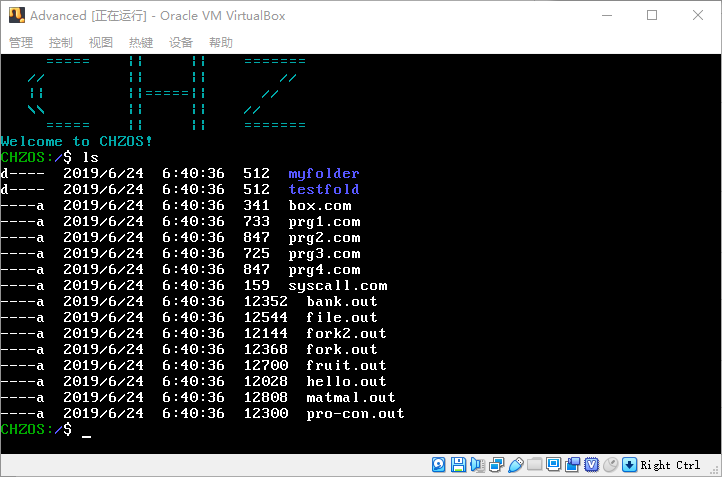
\includegraphics[width=0.8\linewidth]{fig/ls1.png}\\
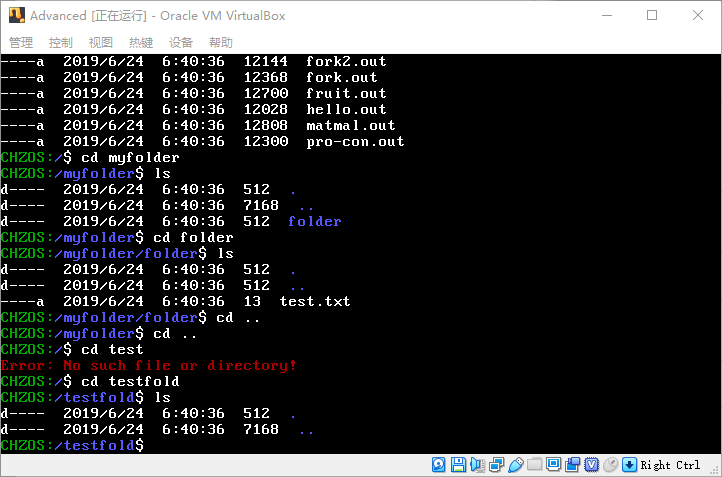
\includegraphics[width=0.8\linewidth]{fig/ls2.png}
\end{tabular}
\caption{目录切换与目录查看}
\label{fig:dir}
\end{figure}

图\ref{fig:hello}展示了上一次实验的多线程程序能够正常执行。
这里涉及到\textbf{FAT12的文件索引、多簇的文件读入、ELF文件的解析、进程的创建与执行、多线程管理}等多个内容,非常复杂,但我的操作系统依然能够正常运行!
\begin{figure}[H]
\centering
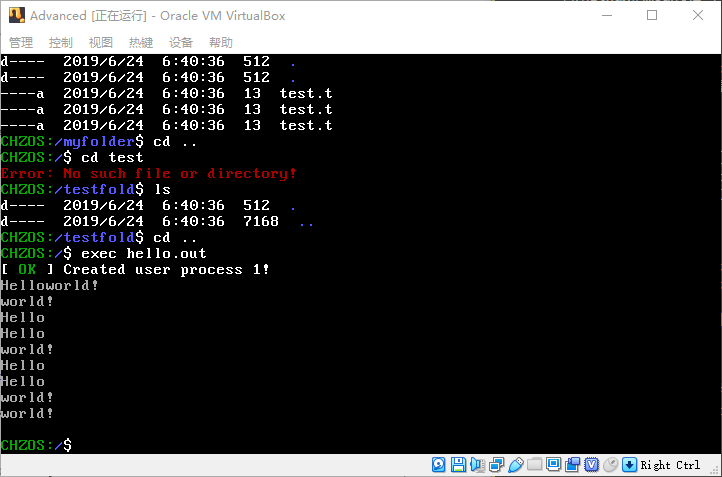
\includegraphics[width=0.8\linewidth]{fig/exec.png}
\caption{正常加载并执行多线程程序}
\label{fig:hello}
\end{figure}

下面的用户程序\verb'file.c'将测试文件的基本功能。
先创建一个文件\verb'testmsg.txt',然后往里面写内容,最后读出并关闭文件。
\begin{lstlisting}
#include "stdio.h"
#include "file.h"

int main()
{
    // Declare the file pointer 
    FILE* fp;

    // Get the data to be written in file 
    char dataToBeWritten[50] = "This is a test message!"; 
  
    // Open the non-existing file with fopen()
    fp = fopen("testmsg.txt", "w");

    // Check if this fp is null 
    // which maybe if the file does not exist 
    if (fp == NULL)
    {
        printf("testmsg.txt file failed to open!"); 
    }
    else
    {

        printf("The file is now opened.\n");

        // Write the dataToBeWritten into the file 
        if (strlen(dataToBeWritten) > 0) 
        {
            // writing in the file using fputs()
            fputs(dataToBeWritten, fp);
            // fputs("\n", fp);
        }

        char dataToBeRead[50];
        fgets(dataToBeRead,strlen(dataToBeWritten),fp);
        dataToBeRead[strlen(dataToBeWritten)] = '\0';

        printf("========= Data read out =========\n\n");
        printf("%s\n\n", dataToBeRead);
        printf("=================================\n\n");

        // Closing the file using fclose()
        fclose(fp);

        printf("Data successfully written in file testmsg.txt\n"); 
        printf("The file is now closed.\n");
    }
    return 0;
}
\end{lstlisting}

\begin{figure}[H]
\centering
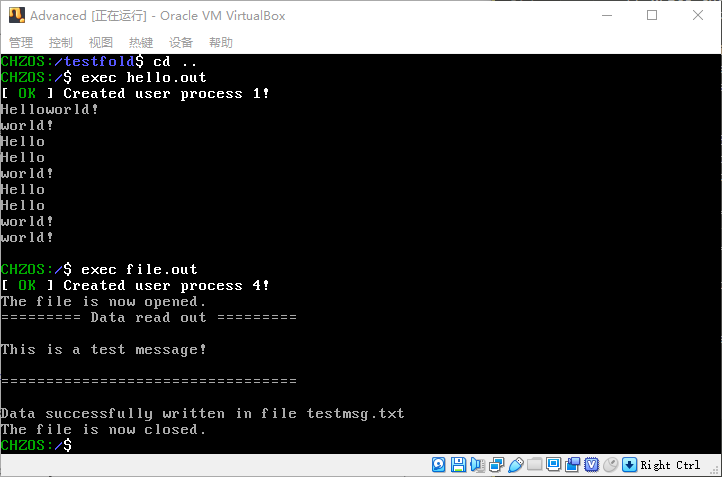
\includegraphics[width=0.8\linewidth]{fig/cfile.png}
\caption{C程序输出结果,注意Data read out那一段是文本写入文件后再读出来的,可以看到结果正确}
\label{fig:cfile}
\end{figure}
\begin{figure}[H]
\centering
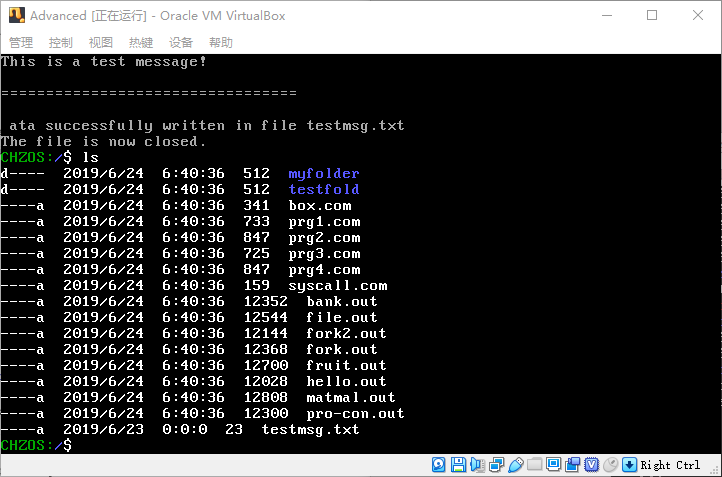
\includegraphics[width=0.8\linewidth]{fig/cfile-ls.png}
\caption{程序结束后查看目录,确实存在新的文件testmsg.txt,由于没有外部时钟的支持,故这里我给文件创建设置的时间会存在不准确,但不影响整体的正确性}
\label{fig:testmsg}
\end{figure}
\begin{figure}[H]
\centering
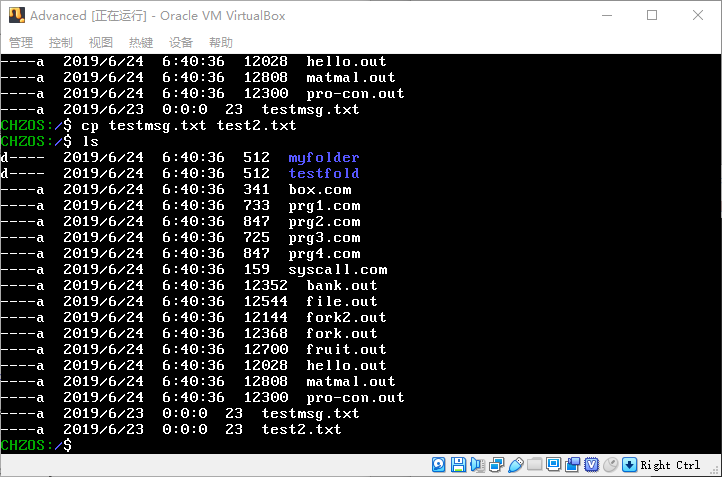
\includegraphics[width=0.8\linewidth]{fig/cfile-cp.png}
\caption{拷贝一份文件test2.txt,可以看见文件属性相同,大小也相同}
\label{fig:cfile-cp}
\end{figure}
\begin{figure}[H]
\centering
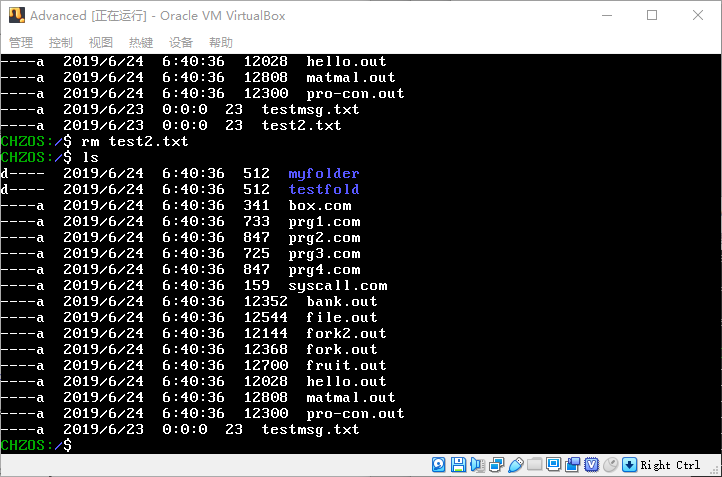
\includegraphics[width=0.8\linewidth]{fig/cfile-rm.png}
\caption{删除该拷贝test2.txt,文件确实从目录中消失了}
\label{fig:cfile-rm}
\end{figure}

上述实验已经将我实施的所有文件操作演示了一遍,均取得了预期的结果。

\section{实验总结}
% 每人必需写一段,文字不少于500字,可以写心得体会、问题讨论与思考、新的设想、感言总结或提出建议等等。不得抄袭,否则按作弊处理。
单是一个文件系统就增加了我操作系统近2000行代码,足以见得文件系统的工程量之大。
而且网上几乎没有合适的参考资料,因为每个操作系统的底层都不一样,对文件系统的实施也就完全不一样。
其实文件系统并不难,按部就班进行实施就好了。
但有很多细节需要注意,一不小心操作系统很可能就会崩溃,毕竟所有的文件读写、执行都是建立在文件系统之上的。

由于Windows 10的子系统WSL不支持FAT12的\verb'mount'操作,故我只能将我的操作系统放上云服务器上进行调试,来来回回折腾非常耗费时间,也大大延长了我的调试进度。
不过好在用户程序不太需要进行修改,故只需编译一次,写入虚拟硬盘一次即可(这也是将具体实施与用户API相分离的好处)。

由于时间所限,本次实验的文件系统只实现了一些基本的功能,且还不够完善,还有很多细节未考虑,也还有很多后续工作没完成。
但不管怎样,我的操作系统也算是完成了大部分的功能,差不多要给它画上尾声了。

\section{参考资料}
\textbf{操作系统实现完整资料:}
\begin{enumerate}
	\item OS Development Series, \url{http://www.brokenthorn.com/Resources/OSDevIndex.html}
	\item Roll your own toy UNIX-clone OS, \url{http://www.jamesmolloy.co.uk/tutorial_html/}
	\item The little book about OS development, \url{http://littleosbook.github.io/}
	\item Writing a Simple Operating System from Scratch, \url{http://www.cs.bham.ac.uk/~exr/lectures/opsys/10_11/lectures/os-dev.pdf}
	\item Intel$^{\textregistered}$ 64 and IA-32 Architectures Software Developer's Manual
	\item UCore OS Lab, \url{https://github.com/chyyuu/ucore_os_lab}
	\item CMU CS 15-410, Operating System Design and Implementation, \url{https://www.cs.cmu.edu/~410/}
	\item 李忠,王晓波,余洁,《x86汇编语言-从实模式到保护模式》,电子工业出版社,2013
\end{enumerate}

\textbf{本次实验参考资料:}
\begin{enumerate}
	\item FAT12文件系统之引导扇区结构,\url{http://blog.sina.com.cn/s/blog_3edcf6b80100cr08.html}
	\item FAT12文件系统之数据存储方式详解,\url{http://blog.sina.com.cn/s/blog_3edcf6b80100crz1.html}
	\item An Overview of FAT12, \url{http://www.disc.ua.es/~gil/FAT12Description.pdf}
	\item FAT12实施,\url{https://github.com/imtypist/fat12}
\end{enumerate}

\appendix
\appendixconfig
\section{程序清单}
\subsection{内核核心代码}
\begin{center}
\begin{tabular}{|c|l|l|}\hline
\textbf{序号} & \textbf{文件} & \textbf{描述} \\\hline
1 & \verb'bootloader.asm' & 主引导程序\\\hline
2 & \verb'kernel_entry.asm' & 内核汇编入口程序\\\hline
3 & \verb'kernel.c' & 内核C入口程序\\\hline
4 & \verb'Makefile' & 自动编译指令文件\\\hline
5 & \verb'bootflpy.img' & 引导程序/内核软盘\\\hline
6 & \verb'mydisk.hdd' & 虚拟硬盘\\\hline
7 & \verb'bochsrc.bxrc' & Bochs配置文件\\\hline
\end{tabular}
\end{center}

\subsection{内核头文件}
\begin{center}
\begin{tabular}{|c|l|l|}\hline
\textbf{序号} & \textbf{文件} & \textbf{描述} \\\hline
1 & \verb'disk_load.inc' & BIOS读取磁盘\\\hline
2 & \verb'show.inc' & 常用汇编字符显示\\\hline
3 & \verb'gdt.inc' & 汇编全局描述符表\\\hline
4 & \verb'gdt.h' & C全局描述符表\\\hline
5 & \verb'idt.h' & 中断描述符表\\\hline
6 & \verb'hal.h' & 硬件抽象层\\\hline
6.1 & \verb'pic.h' & 可编程中断控制器\\\hline
6.2 & \verb'pit.h' & 可编程区间计时器\\\hline
6.3 & \verb'keyboard.h' & 键盘处理\\\hline
6.4 & \verb'tss.h' & 任务状态段\\\hline
6.5 & \verb'ide.h' & 硬盘读取\\\hline
7 & \verb'io.h' & I/O编程\\\hline
8 & \verb'exception.h' & 异常处理\\\hline
9 & \verb'syscall.h' & 系统调用\\\hline
10 & \verb'task.h' & 多进程设施\\\hline
11 & \verb'user.h' & 用户程序处理\\\hline
12 & \verb'terminal.h' & Shell\\\hline
13 & \verb'scancode.h' & 扫描码\\\hline
14 & \verb'stdio.h' & 标准输入输出\\\hline
15 & \verb'string.h' & 字符串处理\\\hline
16 & \verb'elf.h' & ELF文件处理\\\hline
17 & \verb'api.h' & 进程管理API\\\hline
18 & \verb'semaphore.h' & 信号量机制\\\hline
19 & \verb'systhread.h' & 线程模型\\\hline
20 & \verb'pthread.h' & 线程管理API\\\hline
21 & \verb'fat12.h' & FAT12文件系统\\\hline
22 & \verb'sysfile.h' & 虚拟文件系统\\\hline
23 & \verb'file.h' & 文件管理API\\\hline
\end{tabular}
\end{center}

\subsection{用户程序}
用户程序都放置在\verb'usr'文件夹中。
\begin{center}
\begin{tabular}{|c|l|l|}\hline
\textbf{序号} & \textbf{文件} & \textbf{描述} \\\hline
1-4 & \verb'prgX.asm' & 飞翔字符用户程序\\\hline
5 & \verb'box.asm' & 画框用户程序\\\hline
6 & \verb'sys_test.asm' & 系统中断测试\\\hline
7 & \verb'fork_test.c' & 进程分支测试\\\hline
8 & \verb'fork2.c' & 进程多分支测试\\\hline
9 & \verb'bank.c' & 银行存取款测试\\\hline
10 & \verb'fruit.c' & 父子祝福水果测试\\\hline
11 & \verb'prod_cons.c' & 消费者生产者模型测试\\\hline
12 & \verb'hello_world_thread.c' & 多线程Hello\_world测试\\\hline
13 & \verb'matmul.c' & 多线程矩阵乘法测试\\\hline
14 & \verb'file.c' & 文件读写测试\\\hline
\end{tabular}
\end{center}

\section{系统调用清单}
\label{sec:syscall}
\begin{center}
\begin{tabular}{|c|c|}\hline
\verb'int 0x80'\textbf{功能号} & \textbf{功能}\\\hline
0 & 输出OS Logo\\\hline
1 & 睡眠100ms\\\hline
10 & \verb'fork'\\\hline
11 & \verb'wait'\\\hline
12 & \verb'exit'\\\hline
13 & \verb'get_pid'\\\hline
20 & \verb'get_sem'\\\hline
21 & \verb'sem_wait'\\\hline
22 & \verb'sem_signal'\\\hline
23 & \verb'free_sem'\\\hline
100 & 返回内核Shell\\\hline
\end{tabular}
\end{center}

\begin{center}
\begin{tabular}{|c|c||c|c|}\hline
\verb'int 0x81'\textbf{功能号} & \textbf{功能} & \verb'int 0x82'\textbf{功能号} & \textbf{功能}\\\hline
0 & \verb'pthread_create' & 0 & \verb'fopen'\\\hline
1 & \verb'pthread_join' & 1 & \verb'fclose'\\\hline
2 & \verb'pthread_self' & 2 & \verb'fread'\\\hline
3 & \verb'pthread_exit' & 3 & \verb'fwrite'\\\hline
&& 4 & \verb'fgets'\\\hline
&& 5 & \verb'fputs'\\\hline
\end{tabular}
\end{center}

\end{document}

% 实验提交内容
% 实验报告:电子版(Word2003的DOC格式或PDF格式)
% 原程序文件及可执行代码程序文件
% 测试输入数据文件和输出数据文件
% 虚拟机软盘映像文件

% 基础实验项目5个和扩展实验7个
% 实验项目,迟交影响成绩评价!
% 工具与环境可由选择,开发新型工具或优化一套开发环境都可加分!
% 一系列基础实验项目必须连续完成,当前项目只能在前一个项目的基础上进行,体现出前后的进化关系,否则要被约谈,证明没有抄袭行为!
% 一个项目可提交多个改进的版本,实现新功能和个性化特征都有利于提高相应项目的成绩。
% 实验项目提交内容用winrar工具整体压缩打包,统一格式命名为:
%	<学号>+<姓名>+<实验项目号>+<版本号>.rar
%	姓名(学号)实验NvX.zip
%	实验报告、项目文件夹、映像文件
%	ftp://172.18.216.232 sysuac 下周六23:59

% 免考
% 条件:实验1~6全部评价AAAAB+B+或相当
% 最终成绩可能范围:75分以上